\documentclass[12pt]{article}
\usepackage[utf8]{inputenc}
\usepackage{graphicx}
\usepackage{amssymb}
\usepackage{amsthm}
\usepackage{amsmath}
\usepackage{mathtools}
\renewcommand{\qedsymbol}{\rule{0.7em}{0.7em}}
\usepackage{tikz}
\usepackage[margin=0.8in]{geometry}
\setlength{\parskip}{1em}
\DeclarePairedDelimiter{\abs}{\lvert}{\rvert}
\DeclarePairedDelimiter{\floor}{\lfloor}{\rfloor}
\usepackage{tikz}
\usetikzlibrary{arrows.meta,positioning}

\usepackage[ruled]{algorithm2e}
\setlength{\algotitleheightrule}{0pt}

\renewcommand{\thesubsection}{\thesection.\alph{subsection}}

\title{CSC303 Assignment 2}
\author{Elias Volonakis, 1003936789}


\begin{document}

\maketitle

\section{}
The only edge we need to change is the edge $(GB, RU)$ from weak to strong. In that case, the network will be strongly balanced. In particular, all triangles that appear in the network either all have strong edges or 1 strong edge and 2 weak edges. Then it must be true that we don't need to add any edges to make the network strongly balanced. 
\newline 
\newline 


\newpage
\section{}
\subsection{}
Recall that node $n$ will forward the message to the friend $f$ that is “closest” to target node $t$, where closeness is measured by grid distance. Then it must be true that node 13 will forward the message to node 75. The reason being is that the distance from node 75 to the target node 89 is closest (5 local edges). From node 75, then local search will traverse only local edges until it reaches the target node 89. In particular, this will be 85, 86, 87, 88, 89. Hence the overall path will be 13, 75, 85, 86, 87, 88, 89.
\subsection{}
The shortest path between node 13 and 89 is 4 edges long. It is: 13, 36, 78, 88, 89. 

\newpage
\section{}
Recall, for a power law curve that the area under the curve from some point $j$ outward is the total volume of sales generated by all items of sales generated by all items of sales-rank $j$ and higher. Since, the retailer has sold 70,000 downloads amongst the first 1000 top downloads, then the following integral must be true, for some $\alpha \in \mathbb{Z}$:
\\ 
\\
$\int_{1}^{1000} \frac{\alpha}{x} dx = (70000)(0.25) \Rightarrow [\alpha \text{ln}(x)]^{1000}_{1} = 17500 \Rightarrow \alpha(1000) = 17500 \Rightarrow \alpha \approx 2533$
\\ \\
With the above calculation, it must be true that the power law is defined by the function $f(x) = \frac{2533}{x}$
\subsection{}
We wish to calculate the number of sales of the most popular download. \\ That will necessarily be $f(1) = \frac{2533}{1} = 2533$ downloads, which is $(2533)(0.25) = \$633.25$.
\subsection{}
We wish to estimate the total number of sales of the top 100 downloads. That is presicely the following integral:
\\ \\
$\int_{1}^{100} \frac{2533}{x} dx = 2533[\text{ln}(x)]^{100}_1 = 2533(\text{ln}(100) \approx 11664$
\\ \\ 
That is the top 100 songs will have 1165 downloads, which is (11664)(0.25) = \$2916.
\subsection{}
The number of downloads follows a power law, since the less popular a song is, the fewer sales it will result in. That is, the first most popular song will sell more than any other. The second most popular song will not sell more than the most song, but it will sell more than any less popular song. This trend will carry on through all song downloads. The trend is a power law and hence, it is clear that the number of downloads is following this power. 
\newpage
\section{}
\subsection{}
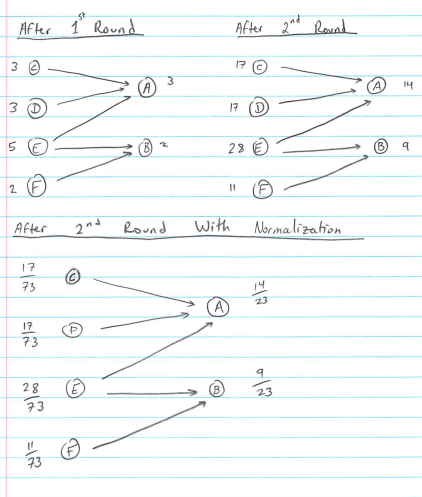
\includegraphics{A2Q4a.PNG}
\subsection{}
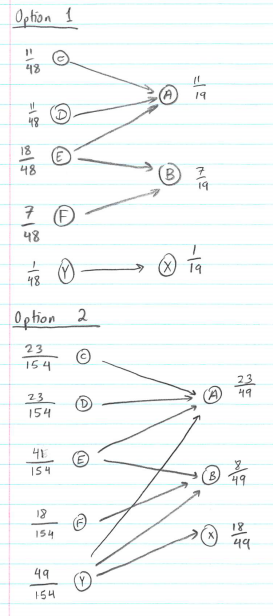
\includegraphics{A2Q4b.PNG}\\
Necessarily then option 2 is best for X
\newpage
\subsection{}
Adding 3 nodes X,Y,Z we wish to maximize the authority score of X. In doing so we must make Y and Z authorities with direct links to X. They must all also have links to all remaining pages A and B. In effect, the values of Y and Z will be greater due to their links to A and B. Those values will be added to the value of X. Thus, the value of X will be maximized. As indicated in the question, the value of X will be second greatest. However, this strategy ought to maximize the authority score of X, as required. 
\newpage
\section{}
\subsection{}
After running the two-step hub authority computation we have the following values:
\\ \\
A1 = A2 = A3 = 243 \\
B1 = B2 = B3 = 81 \\
C1 = C2 = C3 = C4 = C5 = 25 \\
D = 25
\subsection{}
Considering the initialization step as $k = 0$, we have the following formulas: 
\\ \\
A1 = A2 = A3 = $3^{2k+1}$ \\
B1 = B2 = B3 = $3^{2k}$ \\
C1 = C2 = C3 = C4 = C5 = $5^k$ \\
D = $5^k$
\subsection{}
As $k$ goes to infinity we may identify the converged normalized values as follows:
\\
\\
A1 = A2 = A3 = $\lim_{k\to\infty} \frac{3^{2k+1}}{3^{2k+2}+5^{k+1}} = \frac{1}{3}$
\\
\\
B1 = B2 = B3 = $\lim_{k\to\infty} \frac{3^{2k}}{3^{2k+1}+5^{k}} = \frac{1}{3}$
\\
\\
C1 = C2 = C3 = C4 = C5 = $\lim_{k\to\infty} \frac{5^k}{3^{2k+2}+5^{k+1}} = 0$
\\
\\
D = $\lim_{k\to\infty} \frac{5^k}{3^{2k+2}+5^{k}} = 0$
\\ 
\\
This question began with the intuition suggested in the opening paragraph: "One of the basic ideas behind the computation of hubs and authorities is to distinguish between pages that have multiple reinforcing endorsements and those that simply have high in-degree." The graph with the A and B nodes all have multiple reinforcing endorsements from each of the pages and the graph with the C and D nodes are of the latter case. That is, as k goes to infinity, the values of the A and B nodes are $\frac{1}{3}$ since they have multiple reinforcing endorsements. As k goes to infinity, the values of C and D are 0 since they don't have multiple reinforcing endorsements; D simply has a high vertex degree. 


\newpage
\section{}
We wish to compute some subset of people who have the maximum benefit in the context of the campaign. There are stochastic models to consider for this. They are the 1. Linear Threshold Model and 2. Independent Cascade Process. The algorithm that we should implement is a greedy strategy to iteratively add one new initial adopter $v$, so as to maximize the expected marginal gain $f(S+v) - f(S)$, where the function $f(S)$ is defined by the linear threshold model or the independent cascade process as outlined below:
\newline 
\newline 
\textbf{Linear Threshold Model}
\\
We require an edge-weighted network where $w(u,v)$ represents the relative influence of node $u$ on node $v$. In our case such a value should be (Vertex Degree) / (Total Vertex). Each node also has some randomly chosen threshold $q(v) \in [0,1]$. A node will decide to vote for the candidate is the sum of all edge weights into $v$ exceeds the randomly chosen $q(v)$. In each step $t$ a node $v$ is infected if the weighted sum on incident edges coming from infected neighbours exceeds $q(v)$. This is how we get the final set S of adopters satisfying monotonicity and submodularity. 
\\
\\
\textbf{Linear Threshold Model}
\\
We require an edge-weighted network where $w(u,v)$ represents the relative influence of node $u$ on node $v$. In our case such a value should be (Vertex Degree) / (Number of Total Vertices). Each node also has some randomly chosen threshold $q(v) \in [0,1]$. A node will decide to vote for the candidate is the sum of all edge weights into $v$ exceeds the randomly chosen $q(v)$. In each step $t$ a node $v$ is infected if the weighted sum on incident edges coming from infected neighbours exceeds $q(v)$. This is how we get the final set S of adopters satisfying monotonicity and submodularity. 
\\
\\
\textbf{Independent Cascade Process}
We require an edge-weighted network where edge-weights $p(u,v) \leq 1$ represent the probability that node $u$ will influence node $v$. In our case such a value should be (Vertex Degree) / (Number of Total Vertices). In each step $t$ a node that is visited by the politician at step $t-1$ infects each of their uninfected neighbours independently with probability $p(u,v)$. This is how we get the final set S of adopters satisfying monotonicity and submodularity. 






\newpage
\section{}
Individually, all calculations will be shown for each individual in the contact network.
\newline 
\newline 
$\textbf{Person A}$ \\
Person A will be infected on day 0 and becomes contagious on day 1. It is then trivial that the the probability of a getting sick is 1. 
\\
\\
$\textbf{Person B}$\\
Person B can be infected during [3,8] by A. That is 6 days of possible  infection. Note that B cannot be infected by H since H cannot become contagious until day 11, which is outside the [1,2] provided range. The probability of person B getting infected by A is necessarily \\ 1 - P(B does not get infected) = 1 - $\big( \frac{1}{2} \big)^6 = \frac{63}{64}$. 
\\
\\
$\textbf{Person C}$ \\
Person C can be infected during [9,12] by A. That is 4 days of possible infection. Then the probability of person C getting infected by A is necessarily 1 - P(C does not get infected) = 1 - $\big( \frac{1}{2} \big)^4 = \frac{15}{16}$.
\\
\\
$\textbf{Person D}$\\
Person D could get the infection via person C during [6,10], yet the earliest D could be contagious is 10. So then the probability of person D getting sick is necessarily \\ P(C contagious on day 10) $\cdot$ P(D gets infected by D) = $\frac{1}{2} \cdot \frac{1}{2} = \frac{1}{4}$
\\
\\
$\textbf{Person E}$ \\
Person E could get the infection via person B during [5,6]. To get person E infected, B must be contagious by day 6. That said, we may think of the probability of E getting infected as follows:
\\ P(E gets infected via B)  
\\ = $\frac{1}{2}$P(B becomes infected on day 3 or 4) + $\frac{1}{2}$P(B becomes infected on day 5) 
\\ = $\frac{1}{2}$(1-P(B does not become infected day 3 or 4)) + $\frac{}{}$P(B does not get infected on day 3 or 4)P(B gets infected on day 5)
\\ = $\frac{1}{2}(1 - \big( \frac{1}{2} \big)^2) + \frac{1}{2}(1 - \big(\frac{1}{2} \big)^2) \big( \frac{1}{2} \big) = \frac{3}{16}$
\\
\\
$\textbf{Person F}$\\
Person F could become infected via person E during [6,8]. For this to occur, person E must be contagious by day 6. Then necessarily the probability F will become sick is $\frac{1}{2}$P(E becomes sick) = $\frac{3}{32}$
\\
\\
$\textbf{Person G}$
Person G could become infected via person F during [7,9]. For this to occur F could be sick during days 7 or 8. However, F can only become infected on day 6 by E. So then the calculation is as follows: \\
P(G gets infected) = P(F gets infected) $\cdot$ P(F infects G, given F is infected) = $\frac{3}{32} \big(\frac{1}{2} + \big( \frac{1}{2} \big )^2 \big) = \frac{9}{128}$ 
\\
\\ 
\\
\\ 
\\
\\
$\textbf{Person H}$ \\
Person H could become infected by C during [10,11]. For this to occur, C must become infected by A on day 9 or 10. So then the calculation is as follows:
\\
P(H gets infected) = \\ P(C gets infected day 9) $\cdot$ P(H gets infected day 10 or 11) + P(C gets infected day 10) $\cdot$ P(H gets infected day 11) = \\ $\frac{1}{4} \cdot \frac{1}{4} + \frac{1}{2} \cdot \frac{1}{2} = \frac{5}{16}$
\\
\\
$\textbf{Person J and K}$
Neither of these individuals will become infected. As noted above, the earliest H could become infected is day 10. This is after the period [6,8], in which H can infect person J. Thus H will never be able to infect person J. Person J will likewise then never be able to infect person K. So neither person J and K will become infected, so their probability is 0.


\end{document}
